\section{第六章\quad 热力学第二定律}

% 1到9

\pt{热力学第二定律的两种表述}：
\pt{克劳修斯表述}：热量不可能自发地、不花代价地从低温物体传向高温物体。
\pt{开尔文表述}：不可能制造一种循环热机，只从单一热源吸热并把它全部转化为功，而不在外界留下任何影响。

\divider

\pt{卡诺循环}是工作在两个恒温热源之间的可逆循环，由两个\pt{可逆等温过程}和两个\pt{可逆绝热过程}组成。正向卡诺循环过程：绝热压缩、等温吸热、绝热膨胀、等温放热。

卡诺热机效率定义为 $\eta_t=\frac{w_{\mathrm{net}}}{q_1}=1-\frac{q_2}{q_1}=\frac{(T_H-T_L)\Delta s}{T_H\Delta s}=1-\frac{T_L}{T_H}$；逆向卡诺制冷循环的制冷系数 $\varepsilon_c=\frac{q_c}{w_{\mathrm{net}}}=\frac{T_c\Delta s}{(T_0-T_c)\Delta s}=\frac{T_c}{T_0-T_c}$； 逆向卡诺供暖循环的供暖系数：$\varepsilon_c'=\frac{q_1}{w_{\mathrm{net}}}=\frac{T_R\Delta s}{(T_R-T_0)\Delta s}=\frac{T_R}{T_R-T_0}>1$; 概括性卡诺循环通过回热、极限回热等方式，使吸热和放热的平均温度关系等效于卡诺循环，效率仍可写为 $\eta_t=1-\frac{T_L\Delta s_{12}}{T_H\Delta s_{34}}=1-\frac{T_L}{T_H}=\eta_c$；多热源可逆循环中定义平均吸热或放热温度

\pt{卡诺定理 1}：在相同 $T_H$ 和 $T_L$ 之间工作的一切可逆循环，热效率相等，与循环种类和工质无关。\pt{卡诺定理 2}：在相同 $T_H$ 和 $T_L$ 之间工作的一切不可逆循环，热效率小于可逆循环热效率 $q=\int_1^2T\,\mathrm{d}s=T_m(s_2-s_1),T_m=\frac{\int_1^2T\,\mathrm{d}s}{s_2-s_1}$，效率为 $\eta_t=1-\frac{q_2}{q_1}=1-\frac{T_{m,2}}{T_{m,1}}$

\divider

\pt{熵} $s$ 是状态参数；其变化只与初终态有关，与过程路径无关。
对\pt{可逆过程}，熵的定义式为 $\mathrm{d}s=\left(\frac{\delta q}{T}\right)_{\mathrm{rev}}$，对任意可逆循环，克劳修斯积分等式为 $\oint \frac{\delta q}{T_r}=0$。
综合可逆与不可逆循环：$\oint \frac{\delta q}{T_r}\leq 0$。

第二定律的过程表达式为 $s_2-s_1\geq \int_1^2\frac{\delta q}{T_r}$，微分形式为 $\mathrm{d}s\geq \frac{\delta q}{T_r}$

理想气体的玻尔兹曼关系式 $S=k\ln W$

\divider

系统熵变化来源包括热量交换导致的\pt{熵流}、质量交换导致的质熵流，以及不可逆过程导致的熵产闭口系熵方程：$\Delta s=s_{\mathrm{f}}+s_{\mathrm{g}}$。\pt{闭口系熵方程}：$\Delta s=s_{\mathrm{f}}+s_{\mathrm{g}}$ ，$s_{\mathrm{f}}=\int_1^2\frac{\delta q}{T_r}$，$s_{\mathrm{g}}\geq 0$

\divider

\noindent
\begin{minipage}
    [t]{0.48\linewidth}
    \vspace{0pt}
    热源热量的作功能力，即\pt{热量㶲}，为热源放出热量理论上可转化为功的最大部分。对平均放热温度为 $T_{m,H}$ 的热源，热量㶲为 $q_a=\left(1-\frac{T_0}{T_{m,H}}\right)q_1$；热量中不可转化为功的部分为\pt{热量㷻}，$q_{\mathrm{un}}=q_1-q_a=\frac{T_0}{T_{m,H}}q_1=T_0\Delta s_{12}$，$q_a=q_1-T_0\Delta s_{12}$

    冷量指低于环境温度传递的热量，冷量㶲为 $q_a=T_0\Delta s_{12}-q_c$，热量㶲与冷量㶲的计算式相差一个符号；热流与热量㶲同向，冷量与冷量㶲反向
\end{minipage}
\hfill
\begin{minipage}
    [t]{0.48\linewidth}
    \vspace{0pt}
    \centering
    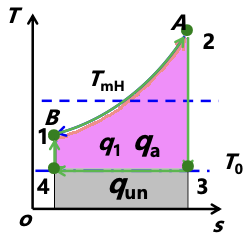
\includegraphics[width=0.8\linewidth]{figures/6热量㶲.png}
    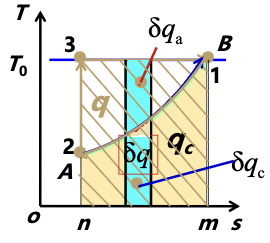
\includegraphics[width=0.8\linewidth]{figures/6冷量㶲.png}
\end{minipage}

\noindent
\begin{minipage}
    [t]{0.48\linewidth}
    \vspace{0pt}
    \pt{闭口系热力学能㶲}：工质因为其状态不同于环境所具备的作功能力，通常是指系统只与环境交换热量可逆过渡到与环境平衡状态作出的最大有用功。
\end{minipage}
\hfill
\begin{minipage}
    [t]{0.48\linewidth}
    \vspace{0pt}
    \centering
    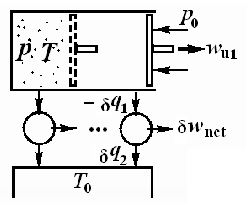
\includegraphics[width=0.8\linewidth]{figures/6热力学能㶲.png}
\end{minipage}

\pt{闭口系热力学㶲}为 $e_{\mathrm{x},U}=u-u_0+p_0(v-v_0)-T_0(s-s_0)$，闭口系从状态 $1$ 到状态 $2$ 的最大有用功：$w_{u,\max,1-2}=e_{\mathrm{x},U,1}-e_{\mathrm{x},U,2}=u_1-u_2-T_0(s_1-s_2)+p_0(v_1-v_2)$

\pt{稳流工质的焓㶲}从状态 $1$ 到状态 $0$ 为 $e_{\mathrm{x},H}=h-h_0-T_0(s-s_0)$，稳流工质从状态 $1$ 到状态 $2$ 可作出的最大有用功为 $w_{u,\max,1-2}=e_{\mathrm{x},H,1}-e_{\mathrm{x},H,2}=h_1-h_2-T_0(s_1-s_2)$，若考虑动能，物流㶲可写为 $e_{\mathrm{x}}=h_1-h_0-T_0(s_1-s_0)+\frac{1}{2}c_{f,1}^2$

机械能可视为\pt{机械㶲}或功㶲，记为 $E_{\mathrm{x},W}$;

热量或冷量的可用能称为\pt{热量㶲}，记为 $E_{\mathrm{x},Q}$，$e_{\mathrm{x},Q}=q_1-T_0(s_2-s_1)$

\pt{㶲损失}与熵产的关系为 $I=T_0S_{\mathrm{g}}=T_0\Delta S_{\mathrm{iso}}$，适用于所有情况、

\pt{闭口系}㶲平衡方程：$E_{\mathrm{x},Q}-W_u - I =E_{\mathrm{x},U_2}-E_{\mathrm{x},U_1}$

\pt{开口系}㶲平衡方程：$Q-Q_0=H_2-H_1+\frac{m}{2}c_{\mathrm{f}2}-\frac{m}{2}c_{\mathrm{f}1}^2+W_\mathrm{s}$

\divider

㶲不守恒：与孤立系熵只增不减相反，孤立系中的\pt{㶲只减不增};\pt{㶲平衡}总表达：流入系统的各种㶲量之和 $-$ 离开系统的各种㶲量之和 $-$ 不可逆过程造成的㶲损失 $=$ 系统㶲变化量，即 $E_{\mathrm{x},Q}-W_u-I=E_{\mathrm{x},U,2}-E_{\mathrm{x},U,1}$。㶲损失即为作功能力损失，均可以以 $T_0S_\mathrm{g}$ 的形式计算

㶲效率为 $\eta_{\mathrm{ex}}=\frac{E_{\mathrm{x},\mathrm{收益}}}{E_{\mathrm{x},\mathrm{代价}}}=\frac{W_s}{E_{\mathrm{x},1}}=\frac{W_s+E_{\mathrm{x},2}}{E_{\mathrm{x},1}}=\frac{W_s}{E_{\mathrm{x},1}-E_{\mathrm{x},2}}$（\pt{后面三项是不同写法，并不是等式}）

\divider
